\documentclass[a4paper]{jacow}

\usepackage[utf8]{inputenc}
\usepackage[english]{babel}			 
\usepackage[final]{pdfpages}
\usepackage{lmodern}
\usepackage{multirow}
\usepackage{ragged2e}
\usepackage{amsmath, amssymb}
\usepackage{tikz}
\usepackage{xcolor}
\usepackage{siunitx}


% color definitions, mainly derived from the maincolor and black
\definecolor{maincolor}{cmyk}{10,75,0.0,0.0}
\colorlet{sensorcolor}{maincolor}
\colorlet{weightcolor}{maincolor!50}
\colorlet{outerblockcolor}{maincolor!30}

\colorlet{irrelevantcolor}{black!10}
\colorlet{midblockfillcolor}{black!10}
\colorlet{midblockdashedbordercolor}{black!50}

% used tikz librarys
\usetikzlibrary{
  arrows,
  shapes.misc,
  shapes,
}

% style definitions for the block diagram
\tikzstyle{basicblock}=[thick, draw, minimum height=2em]
\tikzstyle{vsinnerblock}=[basicblock, rectangle]
\tikzstyle{cinnerblock}=[basicblock, rounded rectangle]
\tikzstyle{outerblock}=[basicblock, fill=outerblockcolor, text width=5em,text centered, minimum height=20em, rounded corners]
\tikzstyle{midblocks}=[outerblock, draw=midblockdashedbordercolor, fill=midblockfillcolor, minimum height=8em, minimum width=20em, text width=10em]

\begin{document}

\title{Investigation of Nature Inspired Algorithms in a practical context by exploiting the characteristics of Braitenberg Vehicle Concepts}

\author{A. Dorn\thanks{andrea.dorn@uni-rostock.de}, University of Rostock, Rostock, Germany \\
		H. Pommerenke\thanks{hermann.pommerenke@uni-rostock.de}, University of Rostock, Rostock, Germany \\
		T. Steinmetz\thanks{tino.steinmetz@uni-rostock.de}, University of Rostock, Rostock, Germany}
	
\maketitle


\begin{abstract}
   Insert shiny abstract!
\end{abstract}

\section{The Braitenberg Vehicle}

The term Braitenberg vehicle (BV) describes a vehicle which is capable of autonomous movement via two independent motors by considering primitive sensor inputs only.

These sensors typically are proximity or light sensors, but may also include gas, acoustic, and similar sensors for specific applications. Movement is achieved by calculating the motor speed $v$ as a linear combinations of the sensor inputs $I$. Therefore, the values collected by the sensors are multiplied with weights $w$ and superimposed for each motor individually. Equation~(\ref{eq:motorequation}) show this principle, where the index $n\in\{\mathrm{L},\mathrm{R}\}$ describes the corresponding motor and $i=0,\ldots,N-1$ denotes the individual sensor. To ensure a net forward movement, an additional bias $w_{n,\text{bias}}$ is added.
\begin{equation}
	v_{n} = \sum\limits_{i=0}^{N-1} w_{n,i} I_{i} + w_{n,\text{bias}}
	\label{eq:motorequation}
\end{equation}
The BV's behaviour can now be varied by adjusting the weights $w$. Considering a vehicle with $N$ sensors, this requires $2N+2$ weight values to be found, i.e. an optimisation problem in $\mathbb{R}^{2N+2}$.

Assuming a symmetric BV, the problem size can be halved, as the weights of the left motor should be in reverse order to the right motor's weights, and the bias values should be the same:
\begin{align}
	w_{\mathrm{L}, i} = w_{\mathrm{R}, N-i} \nonumber \\
	w_{\mathrm{L},\text{bias}} = w_{\mathrm{R},\text{bias}}.\label{eq:symmetry}
\end{align}

\section{E-Puck as Braitenberg Vehicle}

For this project, the educational robot E-Puck serves as a Braitenberg vehicle. It sports $N=8$ infra red proximity sensors which are used as the above mentioned sensor inputs. Figure~\ref{fig:epuck} shows the symmetric distribution of the sensors and the basic principle of the motor control.

\begin{figure}[hbt]
	\centering
	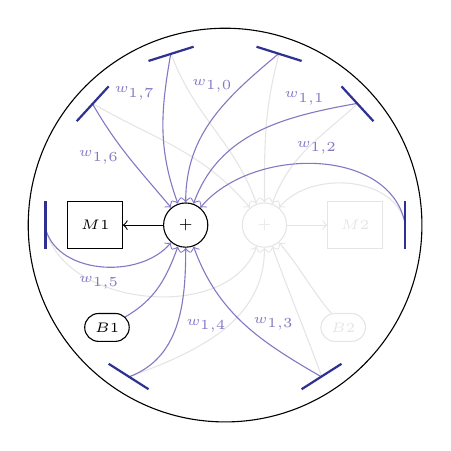
\begin{tikzpicture} 
	\tikzstyle{every node}=[font=\tiny]
	% basic structure
	\draw (0,0) circle [radius=2.5];
	\draw (1.3,-0.3)[irrelevantcolor] rectangle (2,0.3);
	\node ()[irrelevantcolor] at (1.65,0) {$M2$};
	\draw (-1.3,-0.3) rectangle (-2,0.3);
	\node () at (-1.65,0) {$M1$};
	% Adders
	\node (plus1) [draw, shape=circle] at (-0.5,0) {+};
	\draw [->] (plus1) to[out=180, in=0] (-1.3,0);
	\node (plus2) [draw, shape=circle, irrelevantcolor] at (0.5,0) {+};
	\draw [->,irrelevantcolor] (plus2) to[out=0, in=180] (1.3,0);
	% Arrows to second adder
	\draw [->,irrelevantcolor](0:2.29) to[out=100,in=50] (plus2);
	\draw [->,irrelevantcolor](42.5:2.29) to[out=222.5,in=70] (plus2);
	\draw [->,irrelevantcolor](72.5:2.29) to[out=255,in=90] (plus2);
	\draw [->,irrelevantcolor](107.5:2.29) to[out=290,in=110] (plus2);
	\draw [->,irrelevantcolor](137.5:2.29) to[out=330,in=130] (plus2);
	\draw [->,irrelevantcolor](180:2.29) to[out=280,in=250] (plus2);
	\draw [->,irrelevantcolor](237.5:2.29) to[out=20,in=270] (plus2);
	\draw [->,irrelevantcolor](302.5:2.29) to[out=110,in=290] (plus2);
	% Arrows to first adder
	\draw [->,weightcolor](72.5:2.29) to[out=220,in=90] node [near start, left, rotate=0] {$w_{1,0}$} (plus1);
	\draw [->,weightcolor](42.5:2.29) to[out=190,in=70] node [near start, above, rotate=0] {$w_{1,1}$} (plus1);
	\draw [->,weightcolor](0:2.29) to[out=100,in=50] node [midway, above, rotate=0] {$w_{1,2}$} (plus1);
	\draw [->,weightcolor](302.5:2.29) to[out=150,in=290] node [right, rotate=0] {$w_{1,3}$} (plus1);
	\draw [->,weightcolor](237.5:2.29) to[out=20,in=270] node [right, rotate=0] {$w_{1,4}$} (plus1);
	\draw [->,weightcolor](180:2.29) to[out=280,in=230] node [below, rotate=0] {$w_{1,5}$} (plus1);
	\draw [->,weightcolor](137.5:2.29) to[out=300,in=130] node [left, rotate=0] {$w_{1,6}$} (plus1);
	\draw [->,weightcolor](107.5:2.29) to[out=260,in=110] node [near start, left, rotate=0] {$w_{1,7}$} (plus1);
	% Sensors
	\draw [thick, sensorcolor](-7.5:2.3) -- (7.5:2.3);
	\draw [thick, sensorcolor](35:2.3) -- (50:2.3);
	\draw [thick, sensorcolor](65:2.3) -- (80:2.3);
	\draw [thick, sensorcolor](100:2.3) -- (115:2.3);
	\draw [thick, sensorcolor](130:2.3) -- (145:2.3);
	\draw [thick, sensorcolor](172.5:2.3) -- (187.5:2.3);
	\draw [thick, sensorcolor](230:2.3) -- (245:2.3);
	\draw [thick, sensorcolor](295:2.3) -- (310:2.3);
	% Biases
	\node (bias1)[draw,shape=rounded rectangle] at (-1.5,-1.3) {$B1$};
	\draw [->, weightcolor] (bias1) to[out=30, in=250] (plus1);
	\node (bias2)[irrelevantcolor,draw,shape=rounded rectangle] at (1.5,-1.3) {$B2$};
	\draw [->, irrelevantcolor] (bias2) to[out=130, in=310] (plus2);
\end{tikzpicture}
	\caption{Sketch of the E-Puck robot, with motors, sensors and weights of the left side.}
	\label{fig:epuck}
\end{figure}

In the following considerations, the sensor values are normalised to the range of $[0,1]\ni I$, a value of one meaning that an obstacle is at point blank range to the sensor, and zero that no backscattered signal is received at all. The motors' control signals are in the range of $[-1000,1000]\ni v$, with the extreme values meaning full speed forwards and backwards, respectively. Referring to eq.~(\ref{eq:motorequation}), the weights are chosen from the interval $[-1000,1000]\ni w$ accordingly.

In this scenario, the E-Puck shall provide an obstacle avoidance behaviour. Consider the following example as an explanation for the desired functionality: if sensor $I_1$ registers an approaching obstacle (from about 1 o'clock) and therefore generates a value, motor $M_\mathrm{L}$ should reduce it's speed, while $M_\mathrm{R}$ should speed up, which results in a left turn, away from the obstacle.

\section{Evolutionary Approach}

To find (near) optimal values for the weights $w$ with respect to a certain desired behaviour, evolutionary algorithms (EA) can be utilized.

The EA finds an extremal value of a fitness function $f$ over the search space by creating a population of individuals, containing parents and offspring. Each individual holds a genome equal to its position in the search space. In each evolution step, the offspring is formed by copying or \emph{recombining} the parent individuals. The offspring is then randomly\footnote{by a Gaussian $\mathcal{N}(0,\sigma)$ distributed number} \emph{mutated}. The parents for the next generation is selected from the population according to the aforementioned fitness function. The EA strategy can be modified by changing the population size, selection method, mutation and recombination parameters.

In this scenario, a symmetric BV shall show a collision avoidance behaviour while driving around a maze. The search space is formed by the nine weights, thus limited to $[-1000,1000]^9$. The fitness function $f:[-1000,1000]^9\to \mathbb{R}$ has to indicate, how well the BV moves around its environment. Thus, $f$ has to be evaluated over a certain time $T$:
\begin{equation}
	f = \sum\limits_T \tilde{f}.
\end{equation}
While in theory an integration, the total fitness is computed by a sum of multiple fitness contributions over a finite number of time steps. 

The fitness value $\tilde{f}$ of each individual time step should reward directed forward movement, and penalise both close distance to walls and irregular movement: Forward movement corresponds to a high \emph{average} speed between the two motors. In contrast, a high speed \emph{difference} points to irregular movement and many turns. As turning is required to avoid obstacles, this penalty is attenuated with the $\sqrt{\cdot}$ function. The maximum value of the proximity sensor readouts is utilized as an additional penalty. The three aforementioned components are combined via multiplication, which simplifies merging of the different influences\footnote{they have different physical dimensions}. This leads to the following fitness contribution of one time step:
\begin{equation}
	\tilde{f} = \left( v_\mathrm{L} + v_\mathrm{R} \right) \cdot \left( 1 - k_{\Delta v}\sqrt{|v_\mathrm{L}-v_\mathrm{R}|} \right) \cdot \left(1- k_{I} \max\limits_i I_i\right)
	\label{eq:fitness_timestep} 
\end{equation}
The constants $k_{\Delta v}$, $k_I$ prevent the occurrence of negative values for the penalty factors of~(\ref{eq:fitness_timestep}). They also allow for a fine adjustment by weighting the different influences against each other.

In practise, to get an (mostly) unbiased fitness evaluation for each individual, the E-Puck should be placed at the same starting position in the maze manually. The fitness is then evaluated by driving around for a reasonably long time $T$. 

Here, $T\approx\SI{30}{\sec}$ was chosen. For the EA, the $(1+1)$ strategy was tested. A reasonable behaviour was reached after roughly fifty generations.


\section{Adaptive Learning of Individuals}

Due to the random mutation, the EA is a undirected, and therefore relatively slow strategy with to optimise an E-Puck Braitenberg vehicle. The individual makes no learning progress whatsoever, and is eventually killed off by the selection algorithm. Additionally, the learning process heavily depends on the quality of the fitness function.

To achieve a both adaptive and individual learning process, a combination of controller and value system was implemented. The controller provides the basic behaviour by activating the motors according to eq.~(\ref{eq:motorequation}) and the current weights.

The value system's task is to simulate reward and punishment for a certain behaviour by adjusting the weights, as well as the individual's reflexes.

In this specific example, the value systems reacts on a collision with an obstacle.

\end{document}
	